\chapter{Szimuláció}

A szimuláció elsődleges célja egy általános kvantum ismétlő protokoll működésének vizsgálata. Ennek megfelően a különböző fizikai megvalósítások pontos szimulációjától ezek sokszínűsége miatt a továbbiakban eltekintettem, helyette egy általánosított modellen vizsgáltam az egyes paraméterek hatását. A modell elemei a bevezetőnek megfelelően ismétlő állomások és csatornák. Az állomások rendelkeznek kvantum memóriákkal, képesek mérések, és helyi műveletek elvégzésére a memóriájukban tárolt qubitjeiken, valamint egy speciális állomásfajtának tekinthetjük az összefonódott pár forrásokat is. A csatornák az állomásokat összekötő kommunikációs összeköttetések, amelyeken keresztül a qubitjeinket az állomásoknak szétküldjük. Továbbá feltételezzük, hogy az egyes állomások képesek egymás közt hagyományos kommunikációra is. 

\section{Választott környezet, eszközök}

A szimuláció c++ nyelven íródott(c++11-et használ),valamint az Eigen \cite{eigen}  lináris algebra könyvtárt használja. Az elkészítésnél cél volt sokféle szimulációs elrendezés támogatása, emiatt használata a legtöbb esetben egy c++ könyvtáréhoz hasonló. A legegyszerűbb esetben egy előre megírt függvény egyszeri meghívásával akár egy teljes szimuláció is futtatható, viszont a rendelkezésre álló eszközökkel lehetőség van teljesen egyedi szimulációs elrendezés készítésére is. Az egyes elemek 4 fő csoportba sorolhatók, melynek megfelelően az egyes funkciók 4 header fájlba kerültek szétosztásra. Ezek: a kvantumos elemek reprezentációit tartalmazó, az ismétlő protokoll elemeit tartalmazó, a szimuláció vezérléséért felelős, valamint az előre megírt teszteseteket  tartalmazó fájlok.
\section{A szimuláió vezérlése}
A szimuláció vezérlése egy végrehajtási lista alapján történik, melynek kezelését a \texttt{SimRoot} és \texttt{SimItem} osztályok végzik. A lista \texttt{SimItem} típusú elemekből áll. Ebben az osztályban találhatók infromációk az egyes elemek egymáshoz képesti viszonyáról a sorban, valamint a végrehajtandó lépéseket is itt tárolódnak. Egy ilyen lépést egy itt tárolt függvény (std::function) jelképez ami végrehajtáskor meghívódik. Ilyen függvény lehet például egy Bell-mérés végrehajtása, vagy egy qubit átküldése egy csatornán. Ezen felül tárolva van még a végrehajtás tervezett ideje is. A listát kezelő \texttt{SimRoot} osztály ennek alapján új elem felvételénél a megfelelő helyre tudja rakni a tagokat ezzel egy idő szerint rendezett struktúrát hozva létre. A végrehajtásnál így már mindig csak a soron következő  elemmel kell foglalkozni.  Az objektumba felelős még a sor megfelelő ürítéséért is törlésnél, valamint itt található a szimuláció aktuális órája is.
E két osztály a \texttt{Simulation.h} fájlnak része.

\section{A kvantumos elemek reprezentációja}

A szimuláció során elemi kvantumos egységnek nem a kvantum bitet, hanem mivel minden esetben egy vagy több párral kell dolgozni a kvantum bitpárt választottam. Ennek leírására \texttt{qrep.h} fájlban található \texttt{QPair} osztály szolgál. Párt választani alapelemnek abból a szempontból is nagy könnyebség, hogy a két részecske közti lehetséges összefonódást a bitek együttes állapota már tartalmazza, ezért annak külön kezelésével nem kell foglalkozni. Az együttes állapot leírására ennek megfelelően egy 4 dimenziós komplex vektor szolgál(a 2 bit egy 4 dimenziós állapotteret feszít ki).  Ide sorolató továbbá még az egybites kvantumos memóriát reprezentáló \texttt{QMem} osztály. Az egy qubitre való hivatkozáshoz itt tárolva van a pár címe, aminek a tárolt qubit a része, valamint egy index aminek segítségével a összetett páros állapotból ki tudjuk nyerni a számunkra érdekes qubitet. Az objektum tárolni tudja még ezen kívül egy adott qubit beérkezési idejét is, amiből így később számítható a bit teljes memóriában töltött ideje. A két osztál az említetteken túl egyéb szimulációt segítő segédváltozókat tartalmaz még.

\section{Az ismétlő protokoll elemei }

Az ismétlő protokoll működéséhez szükséges elemeket az \texttt{elements.h} fájl tartalmazza. Itt vannak meghatározva a csomópontok, csatornák, valamint az általuk használt eszközök, eljárások. Ezek közül egyik másik erősen épít egymásra. Az itt található fontosabb dolgok ezt is figyelembe véve:\\
\underline{\texttt{Pair2Measure}} osztály ami párokon elvégzendő mérések megvalósítására szolgál. Jelen esetben csak a Bell-mérés megvalósítására szolgál, viszont megfelelő paraméterekkel más mérések is elvégezhetőek. Mérést tud végezni 2 páron.  Ehhez mivel a párok közötti összefonódással számolni is számolni kell létrehozza az így kialakuló minde a két párra kibővített teret és a továbbiakban azon dolgozik. Magát a mérést a bevezetőben leírtak szerint el lehet végezni. Továbbá tartalmaz állítható kisegítő mátrixokat is, amivel például egyszerűbb bázisváltás is végezhető, megfelelő beállításukkal a mérési folyamat tovább egyszerűsíthető. A beépített Bell-mérés(\texttt{.bmeasure()}) ezeket használja, emiatt a beállításuk fontos, viszont ez egyszerűen megtehető egy másik beépített függvénnyel(\texttt{.SetBellMeasure()}).\\
\underline{\texttt{EPR}} osztály, ami összefonódott párok előállításáért felel. Benne állítható a létrehozni kívánt pár(ez bármilyen lehet) állapota, amit itt is egy 4 dimenziós komplex vektor ír le, valamint a kiadott pár ehhez képesti tisztasága, amivel egy ismeretlen zaj hatását lehet imitálni. Beállítható még a pár generálások közt eltelt idő, ami később a szimulációban kerül felhasználásra.\\
\underline{\texttt{Channel}} osztály az egyes csomopontokat összekötő kvantumos kommunikációs csatornák leírására. Az egyes csatornákat a hosszukkal, valamint csillapításukkal, amit itt egy ``csillapítási hosszal'' jellemzünk. A csatorna által okozott zavar/veszteség egy bit egyszeri átküldésénél a legtöbb esetben átviteli valószínűségként nyilvánul meg. Ennek értéke az előző jellemzőkkel leírva:\\
\begin{center}
$ p=e^{-\frac{L}{L_{cs}}}$, ahol $L$ a teljes hossz $L_{cs}$  pedig a ``csillapítási hossz''.\\
\end{center}
Ezeken felül az osztály tartalmaz még a szimulációt segítő egyéb változókat(pl.: melyik két csomópontot köti össze), valamint egy a szimulációs sorban végrehajtandó lépést is. A \texttt{SendThrough} függvény írja le azt, hogy mi történik a qubittel a csatornán való áthaladás során. A csatorna jellemzőinek megfelelően módosítja a qubitet tartalmazó pár állapotat, valamint lépteti tovább a szimulációt azáltal, hogy a végrehajtási sorba beütemezi a következő lépést.\\
\underline{\texttt{Node}} osztály felelős a használt csomópontok leírásáért. El vannak benne tárolva a csomópont működéséhez szükséges információk:  a csomópont helye a felépített kísérleti rendszerben(a többi csomóponthoz képest), a működése során felhasznált eszközök(Bell-mérés, pár létrehozás, pár tisztítás). Ezeken felül minden ilyen csomópont rendelkezik valamennyi memóriával is(\texttt{QMem} tömb) amiken keresztül működése során az egyes qubiteket manipuláln tudja. Az összefonódott párokat létrehozó egységeknél állítható plusz változó még az egyszerre létrehozandó párok száma, valamint a mérést végző egységek esetében a tisztító protokoll által elérendő tisztaság. Az osztályban van még definiálva a végrehajtási sorban fellelhetó szimulációs lépések nagy része is.

\section{Szimuláció működése}

A szimuláció és az alkalmazott modell működésének bemutatásához tekintsük a következő egyszerű esetet. A vizsgált rendszerben két végpont között egy csomópont, valamint két összefonódott pár forrás segítségével szeretnénk összefonódott állapotokat megosztani. Így összesen 5 egységünk és 4 csatornánk van:3 hagyományos csomópont és 2 párt generáló, valamint az őket összekötő csatornák. A továbbiakban egy pár útját vizsgáljuk ahogy halad és változik a rendszerben. Ehhez kiindulásak feltételezzük, hogy már vannak más párok is a rendszerben, viszont a vizsgált párunk számára is van még szabad memória.
\\
\begin{figure}
\centering
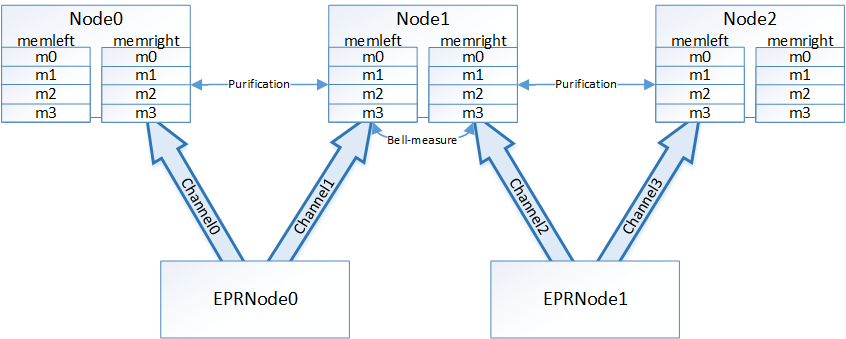
\includegraphics[width=\textwidth,keepaspectratio]{pelda}
\caption[Példa modell egy kisebb hálózatra]{Példa modell egy kisebb hálózatra\\
A vizsgált párt generálja EPRNode0. Ennek megfelelően a hozzá kapcsolódó lépések egy lehetséges sora: \\
1.EPRNode0->GenEPR : A párt létrehozza a forrás.\\
2.Channel0->SendThrough és Channel1->SendThrough: Csatornákon való átküldés\\
3.Node0->ReceiveFromCh és Node1->ReceiveFromCh: Pár qubitjeinek fogadása memóriába\\
4.Node0->ReceiveFromChSuccess és Node1->ReceiveFromChSuccess: Megbizonyosodik arról, hogy mindkét oldal fogadni tudta a pár bitjeit\\
5.Node0->Updateformeasure és Node1->Updateformeasure: Tartalmazó állomások frisstése. Mivel Node0 az egész rendszer egyik végpontja, ezért vele nem lesz több lépés, kívülről vizsgálható, hogy elkészült-e már benne a kívánt összefonódott pár.\\
6/a.Node1-> Bellmeasure: Bell mérés, ha a kétoldali memóriák állapota megfelelő\\
7/a.CorrectAfterMeasure: A pár állapotának javítása a mérési eredménynek megfelelően.\\
8/a.Node0->Updateformeasure és Node2->Updateformeasure: Az új párt tartalmazó két állomás frissítése.\\
6/b.Node1->purification:A memóriák megfelelő állapota esetén az állomáshoz tartozó tisztító protokoll elvégzése.\\
7/b.Node1->Updateformeasure: Állomás frissítése tisztítás után.
}
\end{figure}
\\
A vizsgált párt az egyik párokat generáló csomópont hozza létre a \texttt{GenEPR} lépés segítségével, ami végrehajtása során a pár létrehozásán túl késleltetve ütemezi a következő generálást. Ezen felül ütemezi a hozzá tartozó két csatornán a qubitek átküldésére szolgáló, egyes összekötő csatornák által tárolt \texttt{SendThrough} lépést, a pár megfelelő indexeivel meghívva. Amennyiben a bit átjut a csatornán, a csatorna típusának és hosszának megfelelő késleltetéssel ütemezve lesz a következő lépés ami az egyes csatornák végpontjaihoz tartozó hagyományos csomópontokon végrehajtott \texttt{ReceiveFromCh}. Itt kizárólag azt vizsgáljuk, hogy az éppen beérkező qubit számára van-e hely az egység memóriájában. Amennyiben nincs, a párt megfelelően törli, ha van, akkor pedig berakja az üres memóriába, és ütemezi a következő teendőt, valamint a csomópont struktúrában elfoglalt helyének megfelelően állítja a memória szimulációs állapotát.  Mivel a párral csak akkor tudunk a továbbiakban dolgozni, ha mind a két bitjét sikerrel fogadtuk, ezért a két fogadó csomópontnak ezt a tényt le kell kommunikálniuk klasszikus kommunikációs csatornák segítségével. Ezt a folyamatot jelképezi a megfelelő késleltetéssel ütemezett \texttt{ReceiveFromChSuccess}. Ha mindkét bit sikeresen bekerült a hozzá tartozó memóriába, állít a memória szimulációs állapotán, valamint ütemezi a következő lépést. Ez az \texttt{Updateformeasure} ami egy a csomópontot elvégzett frissítés. Azt nézi, hogy memóriákon végrehajtható-e már a Bell-mérés, valamint hogy mely tárolt párokon szükséges tisztítóprotokollt végrehajtani.
Ennek megfelelően Bell-mérés elvégzést ütemez, vagy tisztítóprotokoll elvégzést ütemez. A Bell-mérés elvégzését a \texttt{Bellmeasure} lépéssel lehet elvégezni. Ennek során a bevezetőben leírtak alapján két páron megtörténik a Bell-mérés. Végeredményül az egyik új pár(a mért bitekből keletkezett) törlődik, míg a két távoli állomás bitjei között új pár keletkezk. A mérésnek 4 eredménye lehet, de mivel a protokoll során mi egy bizonyos állapotot szeretnénk szétosztani szükség van egy mérés utáni korrekcióra. Ehhez szükség van a mérés eredményére, valamint az új pár qubitjein kell elvégezni, ezért itt is fellép a csomópontok között szükséges klasszikus kommunikációból adódó késleltetés. Ez a \texttt{CorrectAfterMeasure} megfelelő időre történő ütemezésével szimulálható. Maga a korrekció elvégezhető a qubiteken történő helyi műveletek végrehajtásával a teleportációs protokoll \cite{bennett1993teleporting} idevágó lépéséhez hasonlóan  Pauli X és Z kapuk segítségével. Legyen a cél állapotunk $\ket{\Phi^+}$. Ekkor a mérés után lehetséges 4 Bell állapotból ez csupán az első biten végrehajtott műveletekkel a következő módon előállítható:
\begin{center}
$\ket{\Phi^+} \rightarrow \ket{\Phi^+}$ \\
$Z\ket{\Phi^-} \rightarrow \ket{\Phi^+}$ \\
$X\ket{\Psi^+} \rightarrow \ket{\Phi^+}$ \\
$ZX\ket{\Psi^-} \rightarrow \ket{\Phi^+}$ \\
\end{center}
Ez után a párt tartalmazó memóriák állapotának frissítése történik, majd a pár qubitjeit tartalmazó állomások frissítése(\texttt{Updateformeasure}). Figyeljük meg, hogy ez a frissítés már a mérés utáni párt tartalmazó állomásokat frissíti, ezáltal az ismétlő protokollban soron következő mérés elvégezhetőségét ezzel a frissítéssel már vizsgáljuk.
Ha egy állomáson elég memória foglalt már, valamint a memóriákhoz tartozó párok tisztasága a mérés előtti előírtnál kisebb, a frissítés ütemezi az állomáshoz tartozó tisztító protokoll elvégzését. Mivel ennek elvégzéséhez két állomás együttműködésére is szükség van, itt is lehet számolni az ebből származó késleltetéssel, továbbá a tisztítás folyamata alatt az érintett memóriákon más feladatot sem végezhetünk. Ezt a programban a tisztítani kívánt memóriák lefoglalásával, majd a tisztítás megfelelő késleltetéssel történő ütemezésével lehet elérni. Ennek megtörténte után az állomás újboli frissítése következik. \\
A működésról általánosan elmondható, hogy alulról fölfele építkezik. Az összes lépés eredő kiváltó ingere az összefonódott párok periodikus létrehozása, amiket a rendszer utána vagy kezel, vagy nem. Egy másik lehetséges megközelítés lehetne, hogy az állomások folyamatosan szabad erőforrásaiknak megfelelően kérnek párokat a forrásoktól, viszont így szükség lenne további klasszikus kommunikáció lebonyolítására, ezért ettől a továbbiakban eltekintettem.

